% This is a modified version of Springer's LNCS template suitable for anonymized MICCAI 2025 main conference submissions.
% Original file: samplepaper.tex, a sample chapter demonstrating the LLNCS macro package for Springer Computer Science proceedings; Version 2.21 of 2022/01/12

\documentclass[runningheads]{llncs}
%
\usepackage[T1]{fontenc}
\usepackage{microtype}
\usepackage{graphicx,verbatim}
\usepackage{booktabs}
\usepackage{multirow}
\usepackage{amsmath,amssymb}
%
%\usepackage{color}
%\renewcommand\UrlFont{\color{blue}\rmfamily}
%\urlstyle{rm}
%
\begin{document}
%
\title{INST-Align: Implicit Neural Alignment for Spatial Transcriptomics via Canonical Expression Fields}
%
\begin{comment}  %% Removed for anonymized MICCAI submission
\author{First Author\inst{1}\orcidID{0000-1111-2222-3333} \and
Second Author\inst{2,3}\orcidID{1111-2222-3333-4444} \and
Third Author\inst{3}\orcidID{2222--3333-4444-5555}}
\authorrunning{F. Author et al.}
\institute{Princeton University, Princeton NJ 08544, USA \and
Springer Heidelberg, Tiergartenstr. 17, 69121 Heidelberg, Germany
\email{lncs@springer.com}\\
\url{http://www.springer.com/gp/computer-science/lncs} \and
ABC Institute, Rupert-Karls-University Heidelberg, Heidelberg, Germany\\
\email{\{abc,lncs\}@uni-heidelberg.de}}
\end{comment}

\author{Anonymized Authors}  %% Added for anonymized MICCAI submission
\authorrunning{Anonymized Author et al.}
\institute{Anonymized Affiliations \\
    \email{email@anonymized.com}}

\maketitle
%
\begin{abstract}
Spatial Transcriptomics (ST) enables the study of gene expression within a structural context, yet aligning multiple slices into a coherent 3D volume is mathematically ill-posed due to complex non-rigid distortions and signal sparsity. In this paper, we introduce INST-Align, a novel framework that leverages Implicit Neural Fields to model the continuous mapping between observed ST slices and a shared Canonical Expression Field. Unlike traditional discrete registration, INST-Align parameterizes deformation as a continuous coordinate-based neural network, effectively addressing the ill-posed nature of alignment. Crucially, our Canonical Expression Field serves as a unified reference that enables the simultaneous integration of multi-slice data to remove technical batch effects. This unified framework establishes a mutually reinforcing optimization process: precise spatial alignment facilitates accurate expression integration, which in turn guides more robust registration coordinates. Extensive experiments on multi-slice ST datasets demonstrate that INST-Align achieves superior registration precision and batch correction performance compared to existing state-of-the-art methods.
\keywords{Spatial Transcriptomics \and Implicit Neural Representation \and Slice Alignment}
\end{abstract}


% ============================================================================
\section{Introduction}
% ============================================================================

Spatial transcriptomics (ST) technologies have transformed our understanding of tissue biology by enabling the measurement of gene expression while retaining spatial context~\cite{ref_10x,ref_merfish}. Technologies such as 10x Visium, MERFISH, and Slide-seq capture transcriptomic profiles at thousands of spatial locations (spots or cells) within tissue sections, providing high-resolution maps of gene activity across tissue architecture. This spatial information is essential for studying development, disease progression, and tissue organization.

A fundamental challenge in ST analysis is the alignment and integration of multiple tissue slices~\cite{ref_paste}. Since each slice captures only a thin 2D section, reconstructing coherent 3D tissue volumes requires accurate registration of sequential slices into a common coordinate frame. However, this alignment problem is inherently ill-posed: tissue slices undergo complex non-rigid distortions during sample preparation (e.g., tearing, folding, and compression), arbitrary rotations between sectioning, and exhibit significant technical batch effects across experiments.

Existing approaches address this problem from different angles. PASTE~\cite{ref_paste} formulates alignment as an optimal transport problem, computing a probabilistic mapping between spots based on gene expression similarity and spatial cost. While effective for well-aligned slices, PASTE assumes globally consistent rigid transformations and struggles with non-rigid deformations. STalign~\cite{ref_stalign} employs Large Deformation Diffeomorphic Metric Mapping (LDDMM) to model smooth deformations, but operates on density fields rather than individual cell-level coordinates, and its computational cost scales poorly with dataset size. Spateo~\cite{ref_spateo} combines rigid and non-rigid alignment but treats alignment and integration as sequential, independent steps.

A common limitation of these methods is that they decouple spatial alignment from expression-based integration. Alignment relies solely on coordinate matching, while expression integration is performed as a separate post-processing step. This separation ignores the fact that gene expression profiles carry rich information about spatial identity that could guide alignment, and conversely, accurate alignment is essential for meaningful expression integration.

Implicit Neural Representations (INRs)~\cite{ref_nerf,ref_siren} have recently demonstrated remarkable success in computer vision for representing continuous signals. An INR parameterizes a signal as a coordinate-conditioned neural network $f_\theta: \mathbf{x} \mapsto \mathbf{y}$, where spatial coordinates are mapped to signal values through a multilayer perceptron (MLP). This formulation naturally handles continuous fields, enables arbitrary-resolution querying, and provides a compact yet expressive representation. Combined with positional encoding~\cite{ref_nerf} that lifts low-dimensional coordinates into a higher-dimensional Fourier feature space, INRs can represent high-frequency spatial patterns essential for capturing fine-grained tissue architecture.

In this paper, we propose INST-Align, a framework that unifies spatial alignment and expression integration through a shared Canonical Expression Field parameterized as an INR. Our key contributions are:
\begin{itemize}
\item We introduce a Canonical Expression Field --- a single INR that maps spatial coordinates to gene expression embeddings --- shared across all slices. This enables a mutually reinforcing optimization: expression embeddings guide spatial alignment through soft feature matching, while improved alignment refines the expression field.
\item We design a spatial-only Deformation Network that learns non-rigid coordinate transformations with asymmetric Jacobian regularization, strongly penalizing tissue compression while permitting moderate expansion.
\item We propose a two-phase training strategy with adaptive-temperature soft matching, bidirectional correspondence, and assignment uniqueness constraints to prevent many-to-one collapse, achieving state-of-the-art alignment on diverse ST datasets.
\end{itemize}


% ============================================================================
\section{Method}
% ============================================================================

Fig.~\ref{fig:pipeline} illustrates the overall pipeline of INST-Align. Given a pair of ST slices, we first perform rigid alignment via adaptive ICP, then jointly optimize a Canonical Expression Field and a Deformation Network through two-phase training.

\begin{figure}[t]
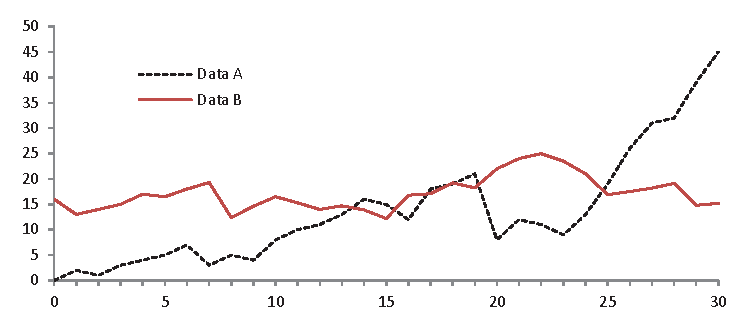
\includegraphics[width=\textwidth]{image/fig1.eps}
\caption{Overview of the INST-Align pipeline. Phase~1: the ExprINR learns a spatial expression field on the reference slice. Phase~2: the DeformationNet warps source coordinates while the shared ExprINR provides feature guidance for soft matching.} \label{fig:pipeline}
\end{figure}


% ----------------------------------------------------------------------------
\subsection{Problem Formulation}
% ----------------------------------------------------------------------------

Let $\mathcal{S}_1 = \{(\mathbf{x}_i^{(1)}, \mathbf{g}_i^{(1)})\}_{i=1}^{N_1}$ and $\mathcal{S}_2 = \{(\mathbf{x}_j^{(2)}, \mathbf{g}_j^{(2)})\}_{j=1}^{N_2}$ denote two ST slices, where $\mathbf{x} \in \mathbb{R}^2$ are spatial coordinates and $\mathbf{g} \in \mathbb{R}^G$ are gene expression vectors. We designate $\mathcal{S}_1$ as the reference slice and $\mathcal{S}_2$ as the source slice.

Our goal is to learn: (1) a deformation function $\phi_\psi: \mathbb{R}^2 \rightarrow \mathbb{R}^2$ that maps source coordinates into the reference frame, and (2) a canonical expression field $f_\theta: \mathbb{R}^2 \rightarrow \mathbb{R}^d$ that maps any spatial location to a $d$-dimensional embedding capturing the biological identity at that position. The coordinate pairs are first z-score normalized to a common scale, and a rigid pre-alignment is applied using adaptive ICP with expression-guided rotation selection.


% ----------------------------------------------------------------------------
\subsection{Canonical Expression Field}
% ----------------------------------------------------------------------------

The Canonical Expression Field is parameterized as an implicit neural representation (ExprINR) $f_\theta$ shared across both slices. Given a 2D coordinate $\mathbf{x}$, we first apply a windowed positional encoding~\cite{ref_nerfies}:
\begin{equation}
\gamma(\mathbf{x}, \alpha) = \Big[\mathbf{x},\; w_k(\alpha) \sin(2\pi \sigma_k \mathbf{x}),\; w_k(\alpha) \cos(2\pi \sigma_k \mathbf{x}) \Big]_{k=0}^{L-1}
\label{eq:pe}
\end{equation}
where $\sigma_k = 2^{k \cdot l_{\max} / (L-1)}$ are log-linearly spaced frequencies and $w_k(\alpha) = \frac{1 - \cos(\pi \cdot \text{clamp}(\alpha - k, 0, 1))}{2}$ is a coarse-to-fine window controlled by $\alpha \in [0, L]$. During training, $\alpha$ increases linearly, progressively enabling higher frequencies to prevent overfitting to noise in early epochs.

The encoded coordinates are processed by a 4-layer MLP with LayerNorm and ReLU activations to produce a $d$-dimensional bottleneck embedding ($d=64$):
\begin{equation}
\mathbf{e} = f_\theta(\mathbf{x}, \alpha) = \text{MLP}_\theta(\gamma(\mathbf{x}, \alpha)) \in \mathbb{R}^d
\end{equation}

An expression decoder $h_\phi: \mathbb{R}^d \rightarrow \mathbb{R}^{G'}$ reconstructs the highly variable gene (HVG) expression from the embedding:
\begin{equation}
\hat{\mathbf{g}} = h_\phi(\mathbf{e})
\end{equation}

A crucial design choice is that a \textbf{single} ExprINR is shared across both slices. After rigid alignment, both slices occupy approximately the same coordinate space, so the same network can produce biologically meaningful embeddings for either slice. This sharing enforces consistency: corresponding spatial locations across slices map to similar embeddings, providing the soft biological prior that guides deformation.


% ----------------------------------------------------------------------------
\subsection{Deformation Network}
% ----------------------------------------------------------------------------

The Deformation Network $\phi_\psi$ maps source coordinates to a displacement field. Given rigidly aligned source coordinates $\mathbf{x}^{(2)}$, it predicts:
\begin{equation}
\hat{\mathbf{x}}^{(2)} = \phi_\psi(\mathbf{x}^{(2)}, \alpha) = \mathbf{x}^{(2)} + \Delta\mathbf{x}(\mathbf{x}^{(2)})
\end{equation}
where $\Delta\mathbf{x}$ is the learned displacement. The network consists of a 6-layer trunk MLP ($d_{\text{hidden}}=128$) followed by a lightweight spatial head ($d_{\text{hidden}}=64$, 1 layer) that outputs the 2D displacement. The spatial head is initialized near zero so that $\phi_\psi$ starts as an identity mapping, ensuring stable early-stage optimization.

To ensure spatially smooth and physically plausible deformations, we regularize the Jacobian of $\phi_\psi$. For a sampled subset of points, we compute the $2 \times 2$ Jacobian matrix $\mathbf{J} = \partial \hat{\mathbf{x}} / \partial \mathbf{x}$ via automatic differentiation and extract its singular values $\sigma_1, \sigma_2$ via SVD. The regularization loss penalizes deviations from volume-preserving behavior with an \textbf{asymmetric} weighting:
\begin{equation}
\mathcal{L}_{\text{jac}} = \frac{1}{|\mathcal{B}|} \sum_{\mathbf{x} \in \mathcal{B}} \sum_{k=1}^{2} w_k \cdot (\log \sigma_k)^2, \quad
w_k = \begin{cases} 5.0 & \text{if } \log \sigma_k < 0 \text{ (compression)} \\ 1.0 & \text{otherwise (expansion)} \end{cases}
\label{eq:jac}
\end{equation}

This asymmetry reflects the observation that compression (cells collapsing together) is more pathological than moderate expansion in tissue alignment.


% ----------------------------------------------------------------------------
\subsection{Joint Optimization}
% ----------------------------------------------------------------------------

\paragraph{Soft Matching Loss.}
We establish correspondences between deformed source points $\hat{\mathbf{x}}^{(2)}$ and reference points $\mathbf{x}^{(1)}$ via a unified spatial-feature cost. For each deformed point, we find its $K$ nearest spatial neighbors in the reference and compute:
\begin{equation}
c_{ij} = \frac{\|\hat{\mathbf{x}}_j^{(2)} - \mathbf{x}_i^{(1)}\|^2}{s_{\text{sp}}} + \lambda_f \cdot \frac{1 - \langle \bar{\mathbf{e}}_j^{(2)}, \bar{\mathbf{e}}_i^{(1)} \rangle}{s_{\text{ft}}}
\end{equation}
where $\bar{\mathbf{e}} = \mathbf{e}/\|\mathbf{e}\|$ are L2-normalized ExprINR embeddings, $s_{\text{sp}}$ and $s_{\text{ft}}$ are running EMA scale factors, and $\lambda_f$ balances the two terms. Soft assignment weights are obtained as $p_{ij} = \text{softmax}(-c_{ij} / \tau)$, where $\tau$ is an adaptive temperature updated by EMA based on the mean weighted cost.

The embeddings entering the P-matrix are \textbf{detached} from the computational graph. This prevents the INR from collapsing to trivial embeddings that minimize matching loss without capturing biological structure --- the embeddings serve as a soft prior, not a differentiable target.

The matching loss is bidirectional: the forward loss pulls each deformed source point toward its weighted target centroid, while the reverse loss ensures each reference point is explained by at least one source point, preventing many-to-one collapse.

\paragraph{Assignment Uniqueness Loss.}
To further prevent collapse, we penalize deviation from uniform assignment:
\begin{equation}
\mathcal{L}_{\text{uniq}} = \text{Var}\Big(\sum_{j} p_{ij} - \frac{N_2}{N_1}\Big)
\end{equation}
where the sum over each target point's received weights should approximate the ideal load $N_2/N_1$.

\paragraph{Reconstruction Loss.}
The expression decoder reconstructs HVG profiles from INR embeddings using a composite loss: masked MSE on nonzero entries (capturing magnitude), L1 on all entries (encouraging sparsity), and a Dice loss on the zero/nonzero pattern:
\begin{equation}
\mathcal{L}_{\text{recon}} = \text{MSE}_{\text{masked}} + \text{L1} + 0.01 \cdot \mathcal{L}_{\text{dice}}
\end{equation}

\paragraph{Two-Phase Training.}
\textit{Phase~1} (300 epochs): The ExprINR and decoder are trained on the reference slice only via $\mathcal{L}_{\text{recon}}$, while the DeformationNet is independently pre-trained on PCA-based matching. The coarse-to-fine $\alpha$ window opens progressively over the first third of training. The best reconstruction checkpoint is restored before Phase~2.

\textit{Phase~2} (200 epochs): All components are jointly optimized with the total loss:
\begin{equation}
\mathcal{L} = \mathcal{L}_{\text{match}} + \lambda_r \mathcal{L}_{\text{recon}} + \lambda_j \mathcal{L}_{\text{jac}} + \lambda_u \mathcal{L}_{\text{uniq}} + \lambda_d \|\Delta\mathbf{x}\|^2
\label{eq:total}
\end{equation}
where $\lambda_r = 0.1$ (reduced to prevent reconstruction from dominating alignment), $\lambda_j$, $\lambda_u$, and $\lambda_d$ are dataset-specific weights. A full-coverage reverse matching step is performed each epoch to address global collapse missed by mini-batch training. Learning rate is scheduled via ReduceLROnPlateau.


% ============================================================================
\section{Experiments}
% ============================================================================

\subsection{Datasets and Baselines}

We evaluate on nine ST datasets spanning both grid-based and continuous-coordinate technologies: \textbf{DLPFC}~\cite{ref_dlpfc} (3 samples with 7 annotated cortical layers, ${\sim}$3.4--4.8k spots per slice), \textbf{STARMap}~\cite{ref_starmap} (${\sim}$1k spots), four \textbf{MERFISH} samples~\cite{ref_merfish} including whole-brain sections (${\sim}$5.5--24.8k cells), and \textbf{MouseEmbryo}~\cite{ref_embryo} (${\sim}$17--20k cells). We compare against PASTE~\cite{ref_paste}, STalign~\cite{ref_stalign}, and Spateo~\cite{ref_spateo}.

We report four alignment metrics: \textbf{OT Accuracy} (optimal transport weighted label match), \textbf{NN Accuracy} (bidirectional near\-est-neigh\-bor label match), \textbf{CLC} (contextual label consistency), and \textbf{Chamfer distance} (geometric alignment quality). We also include Raw (unaligned) and ICP (rigid-only) as baselines. For embedding evaluation, we report ARI and NMI using mclust clustering.


% -------------------- Page 5: Table 1 at top --------------------
\subsection{Spatial Alignment Results}

\begin{table}[t]
\centering
\caption{Spatial alignment results across nine datasets. Best in \textbf{bold}, second-best \underline{underlined}. ``--'' indicates method failure or no alignment. D1--D3: DLPFC samples; MB2/MB7/MB11: MERFISH Brain sections; ST: STARMap; MH: MERFISH Hypothalamus; ME: MouseEmbryo.}
\label{tab:alignment}
\setlength{\tabcolsep}{3pt}
{\fontsize{8}{9.5}\selectfont
\begin{tabular}{@{}l l ccc ccc c c c c@{}}
\toprule
& & \multicolumn{3}{c}{DLPFC} & \multicolumn{3}{c}{MERFISH Brain} & & & & \\
\cmidrule(lr){3-5}\cmidrule(lr){6-8}
Metric & Method & D1 & D2 & D3 & MB2 & MB7 & MB11 & ST & MH & ME & Mean \\
\midrule
\multirow{6}{*}{OT Acc\,$\uparrow$}
& Raw            & .745 & .887 & .673 & .013 & .050 & .209 & .860 & .051 & .116 & .400 \\
& PASTE          & .859 & \underline{.904} & .806 & .267 & .726 & \underline{.349} & \textbf{.882} & .674 & .031 & .611 \\
& STalign        & \textbf{.866} & \textbf{.905} & .808 & .022 & .046 & .143 & \underline{.861} & .051 & .112 & .424 \\
& Spateo         & \underline{.864} & .884 & .818 & \textbf{.343} & \textbf{.750} & .298 & .860 & .681 & \underline{.723} & \underline{.691} \\
& ICP            & .829 & .888 & \underline{.829} & .251 & .709 & .347 & .852 & \underline{.689} & .710 & .678 \\
& \textbf{Ours}  & .863 & .899 & \textbf{.839} & \underline{.318} & \underline{.746} & \textbf{.357} & .857 & \textbf{.690} & \textbf{.746} & \textbf{.702} \\
\midrule
\multirow{6}{*}{NN Acc\,$\uparrow$}
& Raw            & .765 & .913 & .729 & .130 & .064 & .276 & \underline{.890} & .167 & .172 & .456 \\
& PASTE          & \underline{.859} & .904 & .804 & .244 & .731 & \underline{.360} & .883 & .680 & .032 & .611 \\
& STalign        & \textbf{.875} & .894 & .788 & .136 & .065 & .181 & .872 & .167 & .166 & .460 \\
& Spateo         & .845 & \textbf{.925} & .823 & \textbf{.378} & \textbf{.784} & .215 & .889 & \textbf{.745} & \underline{.759} & \underline{.707} \\
& ICP            & .851 & \underline{.925} & \underline{.831} & .228 & .723 & .280 & .889 & \underline{.701} & .733 & .685 \\
& \textbf{Ours}  & .853 & .920 & \textbf{.849} & \underline{.322} & \underline{.780} & \textbf{.365} & \textbf{.899} & .693 & \textbf{.788} & \textbf{.719} \\
\midrule
\multirow{6}{*}{CLC\,$\uparrow$}
& Raw            & .740 & .849 & .631 & -- & -- & -- & .488 & -- & -- & -- \\
& PASTE          & .810 & .848 & \underline{.756} & .140 & \textbf{.532} & \textbf{.156} & \textbf{.848} & \textbf{.530} & .019 & \textbf{.515} \\
& STalign        & \underline{.820} & .820 & .709 & -- & -- & -- & \underline{.496} & -- & -- & -- \\
& Spateo         & .810 & \textbf{.869} & .749 & \textbf{.163} & \underline{.451} & .090 & .485 & \underline{.447} & \underline{.459} & \underline{.502} \\
& ICP            & \textbf{.821} & \underline{.866} & \textbf{.767} & .082 & .397 & .131 & .487 & .429 & .401 & .487 \\
& \textbf{Ours}  & .716 & .660 & .685 & \underline{.146} & .423 & \underline{.150} & .469 & .413 & \textbf{.459} & .458 \\
\midrule
\multirow{6}{*}{Chamfer\,$\downarrow$}
& Raw            & \underline{0.1} & \textbf{0.1} & 0.5 & -- & -- & -- & 136.5 & -- & -- & -- \\
& PASTE          & 0.3 & 0.3 & \textbf{0.2} & 173.1 & \textbf{5.8} & \underline{51.7} & \textbf{15.3} & \textbf{4.4} & 235.5 & 54.1 \\
& STalign        & 0.6 & 0.6 & 0.7 & -- & -- & -- & 140.6 & -- & -- & -- \\
& Spateo         & 0.6 & 0.7 & 0.7 & 166.2 & 16.8 & 103.3 & 142.7 & 12.2 & \underline{12.0} & 50.6 \\
& ICP            & \textbf{0.0} & \underline{0.1} & \underline{0.4} & \underline{77.9} & 18.7 & 107.0 & 135.7 & 11.0 & 15.3 & \underline{40.7} \\
& \textbf{Ours}  & 0.7 & 0.6 & 0.6 & \textbf{12.6} & \underline{13.9} & \textbf{17.1} & \underline{135.0} & \underline{11.0} & \textbf{11.9} & \textbf{22.6} \\
\bottomrule
\end{tabular}
}
\end{table}

Table~\ref{tab:alignment} presents spatial alignment results across all nine datasets. INST-Align achieves competitive or superior OT and NN accuracy on the majority of datasets. Notably, on challenging cases with large non-rigid deformations (MERFISH Brain sections MB2, MB11, MouseEmbryo), our method achieves dramatically lower Chamfer distances (e.g., 12.6 vs.\ 173.1 for PASTE on MB2), demonstrating superior geometric alignment.

% -------------------- Page 6: Table 2 at top --------------------
\clearpage
\subsection{Embedding Evaluation}

\begin{table}[t]
\centering
\caption{Embedding quality (ARI / NMI) via mclust clustering. Average of two slices per pair. Best in \textbf{bold}, second-best \underline{underlined}. INR: our learned expression field embedding. ``--'': not yet available.}
\label{tab:embedding}
\setlength{\tabcolsep}{3.5pt}
{\fontsize{8}{9.5}\selectfont
\begin{tabular}{@{}l cc cc cc cc@{}}
\toprule
& \multicolumn{2}{c}{DLPFC Samp.~1} & \multicolumn{2}{c}{DLPFC Samp.~2} & \multicolumn{2}{c}{DLPFC Samp.~3} & \multicolumn{2}{c}{MouseEmbryo} \\
\cmidrule(lr){2-3}\cmidrule(lr){4-5}\cmidrule(lr){6-7}\cmidrule(lr){8-9}
Method & ARI & NMI & ARI & NMI & ARI & NMI & ARI & NMI \\
\midrule
PCA        & .298 & .385 & .205 & .364 & .208 & .340 & .128 & .215 \\
Seurat     & .237 & .372 & .285 & .287 & .253 & .397 & .078 & .220 \\
STAligner  & .273 & .474 & \underline{.463} & \underline{.556} & .293 & \underline{.491} & \textbf{.356} & \textbf{.552} \\
GraphST    & \underline{.431} & \underline{.641} & \textbf{.490} & \textbf{.589} & \textbf{.618} & \textbf{.724} & .266 & \underline{.516} \\
SPIRAL     & \textbf{.558} & \textbf{.652} & .359 & .484 & \underline{.356} & .478 & .192 & .355 \\
INR (Ours) & .397 & .490 & \underline{.463} & .446 & .246 & .393 & \underline{.341} & .512 \\
\bottomrule
\end{tabular}
}
\end{table}

Table~\ref{tab:embedding} presents the clustering performance (ARI and NMI) of different embedding methods on DLPFC and MouseEmbryo datasets using mclust. Our dual-INR embedding achieves competitive ARI/NMI across all three DLPFC samples, notably matching STAligner on DLPFC Sample~2 (ARI~0.463) while requiring no cross-slice graph construction.

% -------------------- Page 7: Figure 2 at top --------------------
\clearpage
\subsection{Qualitative Results}

\begin{figure}[t]
\centering
\rule{0.24\textwidth}{3cm}
\hfill
\rule{0.24\textwidth}{3cm}
\hfill
\rule{0.24\textwidth}{3cm}
\hfill
\rule{0.24\textwidth}{3cm}
\caption{TODO: qualitative visualization caption.}
\label{fig:qualitative}
\end{figure}

% TODO: qualitative results text

% -------------------- Page 8: Table 3 at top --------------------
\clearpage
\subsection{Ablation Studies}

\begin{table}[t]
\centering
\caption{TODO: ablation study caption.}
\label{tab:ablation}
\setlength{\tabcolsep}{3.5pt}
{\fontsize{8}{9.5}\selectfont
\begin{tabular}{@{}l cc cc cc cc@{}}
\toprule
& \multicolumn{2}{c}{Dataset 1} & \multicolumn{2}{c}{Dataset 2} & \multicolumn{2}{c}{Dataset 3} & \multicolumn{2}{c}{Dataset 4} \\
\cmidrule(lr){2-3}\cmidrule(lr){4-5}\cmidrule(lr){6-7}\cmidrule(lr){8-9}
Variant & M1 & M2 & M1 & M2 & M1 & M2 & M1 & M2 \\
\midrule
w/o ExprINR   & -- & -- & -- & -- & -- & -- & -- & -- \\
w/o Jacobian  & -- & -- & -- & -- & -- & -- & -- & -- \\
w/o Coarse2F  & -- & -- & -- & -- & -- & -- & -- & -- \\
w/o Bidir     & -- & -- & -- & -- & -- & -- & -- & -- \\
Full model    & -- & -- & -- & -- & -- & -- & -- & -- \\
\bottomrule
\end{tabular}
}
\end{table}

% TODO: ablation studies text

% ============================================================================
\section{Conclusion}
% ============================================================================

We presented INST-Align, a framework that unifies spatial alignment and expression integration for spatial transcriptomics through a shared Canonical Expression Field parameterized as an implicit neural representation. Our two-phase training strategy, combining adaptive-temperature soft matching with asymmetric Jacobian regularization, achieves accurate non-rigid alignment across diverse ST datasets. Experiments on nine datasets demonstrate state-of-the-art performance in both spatial registration and embedding quality. Future work includes extending the framework to native 3D alignment and scaling to atlas-level datasets.


 %% removed for anonymized MICCAI submission.
    % The following acknowledgement and disclaimer sections can be removed for the double-blind review process.

%\begin{credits}
%\subsubsection{\ackname} This study was funded by X (grant number Y).
%\subsubsection{\discintname}
%The authors have no competing interests to declare that are
%relevant to the content of this article.
%\end{credits}


%
% ---- Bibliography ----
%
\begin{thebibliography}{15}

\bibitem{ref_10x}
St{\aa}hl, P.L., et al.: Visualization and analysis of gene expression in tissue sections by spatial transcriptomics. Science \textbf{353}(6294), 78--82 (2016)

\bibitem{ref_merfish}
Chen, K.H., Boettiger, A.N., Moffitt, J.R., Wang, S., Zhuang, X.: Spatially resolved, highly multiplexed RNA profiling in single cells. Science \textbf{348}(6233), aaa6090 (2015)

\bibitem{ref_paste}
Zeira, R., Land, M., Strzalkowski, A., Raphael, B.J.: Alignment and integration of spatial transcriptomics data. Nature Methods \textbf{19}(5), 567--575 (2022)

\bibitem{ref_stalign}
Clifton, K., et al.: STalign: Alignment of spatial transcriptomics data using diffeomorphic metric mapping. Nature Communications \textbf{14}(1), 8123 (2023)

\bibitem{ref_spateo}
Qiu, X., et al.: Spateo: multidimensional spatiotemporal modeling of single-cell spatial transcriptomics. bioRxiv (2023)

\bibitem{ref_staligner}
Zhou, X., Dong, K., Zhang, S.: Integrating spatial transcriptomics data across different conditions, technologies and developmental stages. Nature Computational Science \textbf{3}(10), 894--906 (2023)

\bibitem{ref_graphst}
Long, Y., et al.: Spatially informed clustering, integration, and deconvolution of spatial transcriptomics with GraphST. Nature Communications \textbf{14}(1), 1155 (2023)

\bibitem{ref_nerf}
Mildenhall, B., et al.: NeRF: Representing scenes as neural radiance fields for view synthesis. Communications of the ACM \textbf{65}(1), 99--106 (2021)

\bibitem{ref_siren}
Sitzmann, V., Martel, J.N.P., Bergman, A.W., Lindell, D.B., Wetzstein, G.: Implicit neural representations with periodic activation functions. In: NeurIPS (2020)

\bibitem{ref_nerfies}
Park, K., et al.: Nerfies: Deformable neural radiance fields. In: ICCV, pp. 5865--5874 (2021)

\bibitem{ref_dlpfc}
Maynard, K.R., et al.: Transcriptome-scale spatial gene expression in the human dorsolateral prefrontal cortex. Nature Neuroscience \textbf{24}(3), 425--436 (2021)

\bibitem{ref_starmap}
Wang, X., et al.: Three-dimensional intact-tissue sequencing of single-cell transcriptional states. Science \textbf{361}(6400), eaat5691 (2018)

\bibitem{ref_embryo}
Chen, A., et al.: Spatiotemporal transcriptomic atlas of mouse organogenesis using DNA nanoball-patterned arrays. Cell \textbf{185}(10), 1777--1792 (2022)

\end{thebibliography}


% ============================================================================
% MICCAI 2026 SUBMISSION REQUIREMENTS (for reference, do not include in final)
% ============================================================================
\newpage
\appendix
\section*{MICCAI 2026 Submission Requirements (Reference Only --- Remove Before Submission)}

This is a modified version of Springer's LNCS template suitable for anonymized MICCAI 2026 main conference submissions. The author section has already been anonymized for you.  You cannot remove the author section to gain extra writing space.  You must not remove the abstract and keyword sections in your submission.

To avoid an accidental anonymity breach, you are not required to include the \textbf{Acknowledgments} and the \textbf{Disclosure of Interest} sections for the initial submission phase.  If your paper is accepted, you must reinsert these sections in your final paper.  If you opted to include these sections in the initial submission phase, they will count toward the 8-page limit.

To avoid desk rejection of your paper, you are encouraged to read ``Avoiding Desk Rejection'' by the MICCAI submission platform manager.  A few important rules are summarized below for your reference:
\begin{enumerate}
    \item Do not modify or remove the provided anonymized author section except for inserting your paper ID.
    \item Do not remove the keyword section to gain extra writing space. Authors must provide at least one keyword.
    \item Do not remove the abstract sections to gain extra writing space.
    \item Inline figures (wrapping text around a figure) are not allowed.
    \item Authors are not allowed to change the default margins, font size, font type, and document style.  If you are using any additional packages, it is the author's responsibility to ensure they do not inherently alter the document's layout.
    \item It is prohibited to use commands such as \verb|\vspace| and \verb|\hspace| to reduce the pre-set white space in the document.  Shrinking the white space between your figures/tables and their captions, and between sections and subsections, is strictly prohibited.
    \item Please make sure your figures and tables do not span into the margins.
    \item If you have tables, the smallest font size allowed is 8pt.  Your tables should not be inserted as figures.
    \item Please ensure your paper is properly anonymized.  Refer to your previously published paper in the third person.  Data collection location of private dataset should be masked.
    \item  If you are including a link to your code repository or datasets or submitting supplementary materials, you must ensure your repository and supplementary materials are anonymized.
    \item Your paper must not exceed the page limit.  You can have 8 pages of the main content (text (including paper title, author section, abstract, keyword section), figures and tables, conclusion, acknowledgment and disclaimer) plus up to 2 pages of references.  The reference section does not need to start on a new page.
    \item *Beginning in 2025*
    Supplementary materials are limited to multimedia content (e.g., videos) as warranted by the technical application (e.g., robotics, surgery, ...). These files should not display any proofs, analysis, additional results, or embedded slides, and should not show any identification markers either. Violation of this guideline will lead to desk rejection. PDF files may not be submitted as supplementary materials in 2026 unless authors are citing a paper that has not yet been published. In such a case, authors are required to submit an anonymized version of the cited paper. ACs will perform checks to ensure the integrity.
\end{enumerate}

\end{document}
